\documentclass{templateNote}
\usepackage{tcolorbox}
\usepackage{hyperref}
\usepackage{amsmath}
\usepackage{amssymb}
\usepackage{soul}
\usepackage{circuitikz}
\usepackage{enumitem}
\usepackage{comment}
\usepackage{tikz}
\usepackage{parskip}
\usetikzlibrary{decorations.pathreplacing} % Para el corchete decorado
\usepackage[absolute,overlay]{textpos}


\begin{comment}
    \begin{textblock}{5}(10, 10)
        \begin{tcolorbox}[colback=green!5!white,colframe=green!75!black,title=Valor actual neto (VAN)]
            \begin{center}
                \begin{equation*}
                    VAN = \sum_{t=0}^{n} \frac{F_t}{(1+i)^t} - I_0
                \end{equation*}
            \end{center}
        \end{tcolorbox}
    \end{textblock}
\end{comment}


\begin{document}
\imagenlogoU{img/logoNGMFormal_sinF.png}
\linklogoU{https://github.com/NicoGomezM} 
% \imagenlogoD{img/logo-ubb-txt-face.png} 
\titulo{Apunte 1}
\asignatura{Formulación y Evaluación de Proyectos}
\autor{
    \indent
    Nicolás {Gómez Morgado}
}


\portada
\margenes 
\tableofcontents
\newpage

\section{Importante}

\begin{itemize}
    \item Es necesario saber calcular porcentajes y tasas de interés, asi como también saber calcular el valor presente y futuro de una inversión.
    \item Es necesario saber calcular el Reajuste dados los valores que se nos entregan.
\end{itemize}

\subsection{Conceptos clave}

\begin{itemize}
    \item \textbf{Proyectos:} Conjunto de actividades interrelacionadas que se realizan para alcanzar un objetivo.
    \item \textbf{Inversión:} Es el desembolso de recursos financieros para la adquisición de bienes y servicios.
    \item \textbf{Rentabilidad:} Es la relación entre los beneficios obtenidos y los recursos invertidos.
\end{itemize}

\newpage
\section{Criterios para evaluar inversiones}
\subsection{Método de evaluación inicial}
\begin{enumerate}[label=\alph*)]
    \item Incluir \textbf{todos los flujos de caja} que ocurren durante la vida del proyecto.
    \begin{center}
        \begin{tikzpicture}
            % Línea de tiempo
            \draw[-] (0,0) -- (10,0);
        
            % Etiquetas
            \node at (0,0.5) {Cuna};
            \node at (10,0.5) {Tumba};
        
            % Marcadores
            \draw (0,0.1) -- (0,-0.1);
            \draw (10,0.1) -- (10,-0.1);
        \end{tikzpicture}
    \end{center}
    \item Considerar el \textbf{valor del dinero} en el tiempo. \\
    Esto se refiere a que el dinero hoy vale más que el dinero en el futuro. Este termino se relaciona casi por completo con el costo de oportunidad.
    \item Incorporar la \textbf{tasa de retorno requerida} en el proyecto.\\
    Se refiere a que el rendimiento económico que promete el proyecto supere mínimamente al rendimiento que generalmente se ofrece por el mercado (métodos de inversion en banca).
\end{enumerate}

\subsection{Criterios comúnmente usados}

\subsubsection{Periodos de recuperacion de inversion (\textit{Payback})}
\begin{itemize}
    \item Numero de años que se requieren para recuperar la inversión inicial.
    \item Tiempo que le toma al proyecto generar suficientes ingresos para autofinanciarse.
    \item Depende de la naturaleza del proyecto y del criterio de los inversionistas determinar si el periodo de recuperación es aceptable. 
\end{itemize}
\textbf{Debilidades:}
\begin{itemize}
    \item \hl{Subjetivo}.
    \item No considera el valor del dinero en el tiempo.
    \item No considera la tasa de retorno requerida.
    \item No considera los flujos de caja después del periodo de recuperación.
\end{itemize}

\subsubsection{Periodo de recuperacion de inversion descontado (\textit{Payback descontado})}
\begin{itemize}
    \item Se calcula descontando los flujos de caja futuros a una tasa de descuento.
    \item Periodo de recuperación se calcula con los flujos netos.
\end{itemize}
\textbf{Debilidades:}
\begin{itemize}
    \item Dependen del criterio del inversionista.
\end{itemize}

\newpage

\begin{tcolorbox}
    \begin{center}
        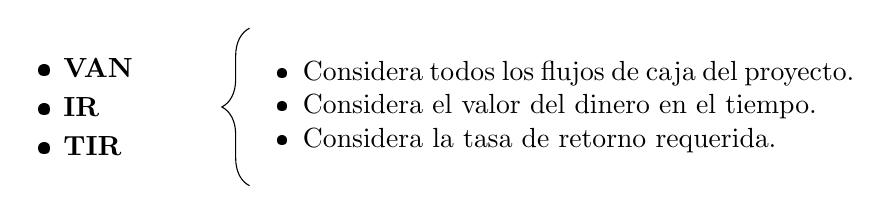
\begin{tikzpicture}
            % Lista de métodos
            \node[anchor=west] (van) at (0,0) {\textbf{• VAN}};
            \node[anchor=west] (ir) at (0,-0.5) {\textbf{• IR}};
            \node[anchor=west] (tir) at (0,-1) {\textbf{• TIR}};
        
            % Corchete
            \draw[decorate,decoration={brace,amplitude=10pt,mirror,raise=5pt},yshift=0pt] (3,0.5) -- (3,-1.5) node [black,midway,xshift=0.8cm] {};
        
            % Características
            \node[anchor=west] at (2.5,-0.5) {
                \begin{minipage}{0.65\textwidth}
                    \begin{itemize}
                        \item Considera todos los flujos de caja del proyecto.
                        \item Considera el valor del dinero en el tiempo.
                        \item Considera la tasa de retorno requerida.
                    \end{itemize}
                \end{minipage}
            };
        \end{tikzpicture}
    \end{center}
\end{tcolorbox}


\subsubsection{Valor actual neto (VAN)}

\begin{align*}
    VAN &= \sum_{t=0}^{n} \frac{\textnormal{FCA}_t}{(1+k)^t} - I_0
\end{align*}

\textbf{Criterios de decisión:}
\begin{itemize}
    \item Si $VAN > 0$, el proyecto es \textbf{aceptable}.
    \item Si $VAN < 0$, el proyecto es \textbf{rechazable}.
\end{itemize}

\subsubsection{Indice de Rentabilidad (IR)}

\begin{align*}
    IR &= \sum_{t=0}^{n} \frac{\textnormal{FCA}_t}{(1+k)^t}/I_0
\end{align*}

\textbf{Criterios de decisión:}
\begin{itemize}
    \item Si $IR \geq 1$, el proyecto es \textbf{aceptable}.
    \item Si $IR < 1$, el proyecto es \textbf{rechazable}.
\end{itemize}

\subsubsection{Tasa interna de retorno (TIR)}

\begin{align*}
    I_0 &= \sum_{t=0}^{n} \frac{\textnormal{FCA}_t}{(1+TIR)^t}
\end{align*}

\textbf{Criterios de decisión:}
\begin{itemize}
    \item Si $TIR > k$, el proyecto es \textbf{aceptable}.
    \item Si $TIR < k$, el proyecto es \textbf{rechazable}.
\end{itemize}

\newpage
\textbf{Ejemplo 1:} Una empresa estudia la posibilidad de emprender un proyecto de inversión de dos años de duración. El proyecto exige la compra de un activo con un desembolso inicial de \$86.000 . Con la actividad que genera dicho activo se esperan unos flujos de caja de \$45.000 el primer año y \$51.000 el segundo año. Se sabe que el tipo de interés del capital o coste del capital es del 6\% anual. Se pide:
\begin{enumerate}[label=\alph*)]
    \item Calcule la Tasa Interna de Retorno (TIR) de la inversión.
    \begin{align*}
        \frac{45000}{(1+TIR)} + \frac{51000}{(1+TIR)^2} &= 86000 \\
        86000 - \frac{45000}{(1+TIR)} - \frac{51000}{(1+TIR)^2} &= 0 \\
        \frac{86000(1+TIR)^2 - 45000(1+TIR) - 51000}{(1+TIR)^2} &= 0 \\
        \frac{86000(1+TIR)^2 - 45000 - 45000TIR - 51000}{(1+TIR)^2} &= 0 \\
        \frac{86000(1+2TIR+{TIR}^2)-45000TIR-96000}{(1+TIR)^2} &= 0 \\
        -10000 + 127000TIR + 86000{TIR}^2 &= 0 \\
        86000{TIR}^2 + 127000TIR - 10000 &= 0 \\
        86{TIR}^2 + 127TIR - 10 &= 0 
    \end{align*}
        \textbf{Resolviendo la ecuación cuadrática:}
    \begin{align*}
        TIR &= \frac{-b \pm \sqrt{b^2 - 4ac}}{2a} \\
        TIR &= \frac{-127 \pm \sqrt{127^2 - 4(86)(-10)}}{2(86)} \\
        TIR &= \frac{-127 \pm \sqrt{16129 + 3440}}{172} \\
        TIR &= \frac{-127 \pm \sqrt{19569}}{172} \\
        TIR &= \frac{12.8892}{172} = 0.07493 \wedge TIR = \frac{-265.8892}{172} = -1,5458 \\
        TIR &= 0.07493
    \end{align*}
    Por lo tanto la TIR es de 7.493\%.
    \item Calcule el VAN.
    \begin{align*}
        VAN &= \frac{45000}{(1+0.06)} + \frac{51000}{(1+0.06)^2} - 86000 \\
        VAN &= \frac{45000}{1.06} + \frac{51000}{1.1236} - 86000 \\
        VAN &= 42452.8301 + 45389.8184 - 86000 \\
        VAN &= 87842.6485 - 86000 \\
        VAN &= 1842.6485
    \end{align*}
    \item Explique si la inversión es aceptable según ambos criterios.
    \\Por lo tanto la inversion es aceptable ya que el VAN es positivo y la TIR es mayor al costo de oportunidad.
\end{enumerate}

\begin{tcolorbox}[colback=purple!5!white,colframe=purple!75!black,title=Importante]
    \begin{itemize}
        \item La TIR es buena herramienta siempre que los flujos sean convencionales. (-+++++...+)
        \item Con multiples cambios de signos se presentan varias TIR. (-++-++-+...+)
        \item La TIR \textbf{solo se usa} con flujos convencionales, en caso contrario se usa el \textbf{VAN}.
    \end{itemize}
\end{tcolorbox}

\textbf{Ejemplo:} Para una empresa con intereses del 15\% anual y con flujos de caja:

\begin{center}
    \begin{tikzpicture}
        % Línea de tiempo
        \draw[->] (0,0) -- (12,0) node[right] {Tiempo};
    
        % % Puntos de tiempo (espaciados más)
        % \foreach \x in {0, 2, 4, 6, 8, 10}
        %     \draw (\x,0.1) -- (\x,-0.1) node[below] {$\x$};
    
        % Flujos de caja (ajustados a los nuevos puntos de tiempo)
        \draw (0,0) -- (0,-0.5) node[below] {(900)};
        \draw (2,0) -- (2,0.5) node[above] {300};
        \draw (4,0) -- (4,0.5) node[above] {400};
        \draw (6,0) -- (6,0.5) node[above] {400};
        \draw (8,0) -- (8,0.5) node[above] {500};
        \draw (10,0) -- (10,0.5) node[above] {600};
    \end{tikzpicture}
\end{center}
Calcular:
\begin{enumerate}[label=\alph*)]
    \item TIR
    \item VAN
    \item IR
\end{enumerate}

\begin{align*}
    900 &= \frac{300}{1-TIR} + \frac{400}{(1-TIR)^2} + \frac{400}{(1-TIR)^3} + \frac{500}{(1-TIR)^4} + \frac{600}{(1-TIR)^5} \\
    &\textnormal{\textit{Calculo en excel:}}\\
    TIR &= 34,372\%
\end{align*}
Por lo tanto el TIR equivale a 34,372\%.

\begin{align*}
    VAN &= \frac{300}{(1+0.15)} + \frac{400}{(1+0.15)^2} + \frac{400}{(1+0.15)^3} + \frac{500}{(1+0.15)^4} + \frac{600}{(1+0.15)^5} - 900 \\
    &\textnormal{\textit{Calculo en excel:}}\\
    VAN &= 510,5161
\end{align*}
Por lo tanto el VAN equivale a 510,5161.

\begin{align*}
    IR &= (\frac{300}{(1+0.15)} + \frac{400}{(1+0.15)^2} + \frac{400}{(1+0.15)^3} + \frac{500}{(1+0.15)^4} + \frac{600}{(1+0.15)^5})/900 \\
    &\textnormal{\textit{Calculo en excel:}}\\
    IR &= 1,5672
\end{align*}

\begin{figure}[H]
    \centering
    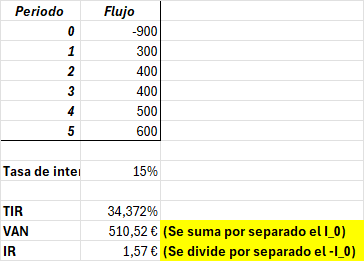
\includegraphics[width=0.5\textwidth]{img/EjemploCalculo.png}
\end{figure}


\subsubsection{Tasa promedio de rendimiento (TPR)}

\begin{itemize}
    \item No considera flujos de caja.
    \item No considera el valor del dinero en el tiempo.
    \item Se basa en la utilidad contable promedio.
    \item Se usa porque es \textbf{fácil de calcular}.
\end{itemize}

\begin{align*}
    TPR &= \frac{\textnormal{Utilidad media}}{\textnormal{Inversión}} * 100
\end{align*}

\begin{tcolorbox}
    \begin{em}
        \begin{center}
            \begin{tabular}{l l}
                Ingresos por ventas & ~ \\
                Costo de ventas & \textcolor{red}{Deprec. y amortiz.} \\
            \end{tabular}
            \rule{11cm}{0.2 mm} \\[0.1 cm]
            \begin{tabular}{l l}
                Margen bruto & ~ \\
                Gastos de adm. y ventas & \textcolor{red}{Deprec. y amortiz.} \\
            \end{tabular}
            \rule{11cm}{0.2 mm} \\[0.1 cm]
            \begin{tabular}{l l}
                Resultado operacional & ~ \\
                Gastos financieros & ~ \\
            \end{tabular}
            \rule{11cm}{0.2 mm} \\[0.1 cm]
            \begin{tabular}{l l}
                Resultados antes de impuestos & ~ \\
                Impuestos a la renta & ~ \\
            \end{tabular}
            \rule{11cm}{0.2 mm} \\[0.1 cm]
            \begin{tabular}{l l}
                Resultado neto & ~ \\
                \textcolor{red}{+ Depreciación y amortización} & ~ \\
            \end{tabular}
            \rule{11cm}{0.2 mm} \\[0.1 cm]
            \begin{tabular}{l l}
                Flujo de caja & ~ \\
            \end{tabular}
        \end{center}
    \end{em}
\end{tcolorbox}

\textbf{Ejemplo:} Para una empresa que invierte \$900 y tiene los mismos flujos de caja que el ejercicio anterior, si esta inversion se deprecia en partes iguales en todos los periodos, calcular la TPR.

\begin{align*}
    TPR &= \frac{\frac{(300-(900/5)) + (400-(900/5)) + (400 -(900/5)) + (500 -(900/5)) + (600 -(900/5))}{5}}{900} \\
    TPR &= \frac{\frac{300-180 + 400-180 + 400-180 + 500-180 + 600-180}{5}}{900} \\
    TPR &= \frac{\frac{120 + 220 + 220 + 320 + 420}{5}}{900} \\
    TPR &= \frac{1300}{5*900} \\
    TPR &= \frac{1300}{4500} \\
    TPR &= 0.2888
\end{align*}

Por lo tanto la TPR es de 28,$\overline{88}$\%.

\rule{\linewidth}{0.1 mm}

\textbf{Ejercicio:} Una empresa tiene \$35000 dispuestos para inversiones, para las inversiones presentadas en la tabla, seleccionar los proyectos que se deben realizar basándose en su costo y VAN proporcionados.

\begin{center}
    \begin{tabular}{|c|c|c|}
        \hline
        Proyecto & Costo & VAN \\
        \hline
        A & 3600 & 380 \\
        B & 2100 & 500 \\
        C & 5800 & 1100 \\
        D & 7200 & 1060 \\
        E & 1060 & 320 \\
        F & 4490 & 1660 \\
        G & 2391 & 1010 \\
        H & 9810 & 2800 \\
        I & 6580 & 650 \\
        J & 1270 & 230 \\
        K & 1290 & 780 \\
        L & 5690 & 1270 \\
        \hline
    \end{tabular}
\end{center}

Conociendo el dinero enfocado en inversiones, se deben seleccionar los proyectos que se deben realizar basándose en su costo y VAN proporcionados. Se debe seleccionar los proyectos que tengan un VAN positivo y que no superen el monto total de la inversión, para hacer esto vamos a calcular el IR de cada proyecto.

\begin{center}
    \begin{tabular}{|c|c|c|c|}
        \hline
        Proyecto & Costo & VAN & IR \\
        \hline
        A & 3600 & 380 & 0.1055 \\
        B & 2100 & 500 & 0.2380 \\
        C & 5800 & 1100 & 0.1896 \\
        D & 7200 & 1060 & 0.1472 \\
        E & 1060 & 320 & 0.3018 \\
        F & 4490 & 1660 & 0.3704 \\
        G & 2391 & 1010 & 0.4223 \\
        H & 9810 & 2800 & 0.2853 \\
        I & 6580 & 650 & 0.0987 \\
        J & 1270 & 230 & 0.1811 \\
        K & 1290 & 780 & 0.6047 \\
        L & 5690 & 1270 & 0.2233 \\
        \hline
    \end{tabular}
\end{center}

Ahora con estos datos ordenaremos los proyectos de mayor a meno IR e iremos sumando sus costos para ver hasta que proyecto podemos llegar.

\begin{center}
    \begin{tabular}{|c|c|c|c|c|}
        \hline
        Proyecto & Costo & VAN & IR & Costo Acumulado\\
        \hline
        K & 1290 & 780 & 0.6047 & 1290 \\   
        G & 2391 & 1010 & 0.4223 & 3681 \\
        F & 4490 & 1660 & 0.3704 & 8171 \\
        E & 1060 & 320 & 0.3018 & 9231 \\
        H & 9810 & 2800 & 0.2853 & 19041 \\
        B & 2100 & 500 & 0.2380 & 21141 \\
        L & 5690 & 1270 & 0.2233 & 26831 \\
        C & 5800 & 1100 & 0.1896 & 32631 \\
        J & 1270 & 230 & 0.1811 & 33901 \\
        D & 7200 & 1060 & 0.1472 & 41101 \\
        A & 3600 & 380 & 0.1055 & 44701 \\
        I & 6580 & 650 & 0.0987 & 51281 \\
        \hline
    \end{tabular}
\end{center}

Por lo tanto los proyectos que se deben realizar son: K, G, F, E, H, B, L, C, J. No se utilizo el total de la inversion ya que para ninguno de los proyectos que quedaban alcanzaba el presupuesto.

\end{document}
